%\documentclass[12pt, twoside, openany]{book}
%chktex-file 1
\documentclass[12pt, oneside]{book}  % jednostranna tlac
\linespread{1.25} % hodnota 1.25 by mala zodpovedat 1.5 riadkovaniu
\pagestyle{plain}
% -------------------
% --- Packages
% -------------------
\usepackage[a4paper,top=2.5cm,bottom=2.5cm,left=3.5cm,right=2cm]{geometry}
\usepackage[utf8]{inputenc}
\usepackage[T1]{fontenc}
\usepackage[slovak]{babel}
\usepackage{graphicx}
\usepackage{url}

% --- additional packages
\usepackage{epsfig}
\usepackage{epstopdf}
\usepackage[chapter]{algorithm}
\usepackage{algorithmic}
\usepackage{listings}
\usepackage{amsmath}
\usepackage{amssymb}
\usepackage{multirow}
\usepackage{booktabs}
\usepackage{color}
\usepackage{setspace}
\usepackage{tabularx}
\usepackage{textcomp}
\usepackage{caption}
\usepackage{natbib}
\usepackage{subcaption}
%\usepackage[font=large]{subcaption}
\usepackage{emptypage}
\usepackage{float}
\usepackage[hidelinks,breaklinks]{hyperref}
%\usepackage{minted}
\usepackage[thinlines]{easytable}
\usepackage{amsmath}
%\captionsetup[subfigure]{font=large}




%aby sa nevykreslovali obrazky
%\renewcommand{\includegraphics}[2][]{
%   \fbox{#2}% print file name in a small box
%}


% -------------------
% --- Definicia zakladnych pojmov
% -------------------
\def\mfrok{2024}
\def\mftitle{Automatická Generácia Úrovní pre Rytmické Počítačové Hry}
\def\mfthesistype{Diplomová práca}
\def\mfauthor{Bc. Filip Masný}
\def\mfskolitel{Ing. Viktor Kocur, PhD.}
\def\mfplacedate{Bratislava, 2024}
\def\mfuniversity{Univerzita Komenského v Bratislave }
\def\mffaculty{Fakulta matematiky, fyziky a informatiky}
\def\mfodbor{18. Informatika}
\def\program{Aplikovaná informatika}
\def\mfpracovisko{Katedra aplikovanej informatiky}

\setcounter{secnumdepth}{2}

\begin{document}
\frontmatter


% -------------------
% --- Obalka ------
% -------------------
\thispagestyle{empty}

\noindent
\begin{minipage}{\textwidth}
    \begin{center}
        \textbf{\mfuniversity \\
            \mffaculty}
    \end{center}
\end{minipage}

\vfill
\begin{figure}[!hbt]
    \begin{center}
        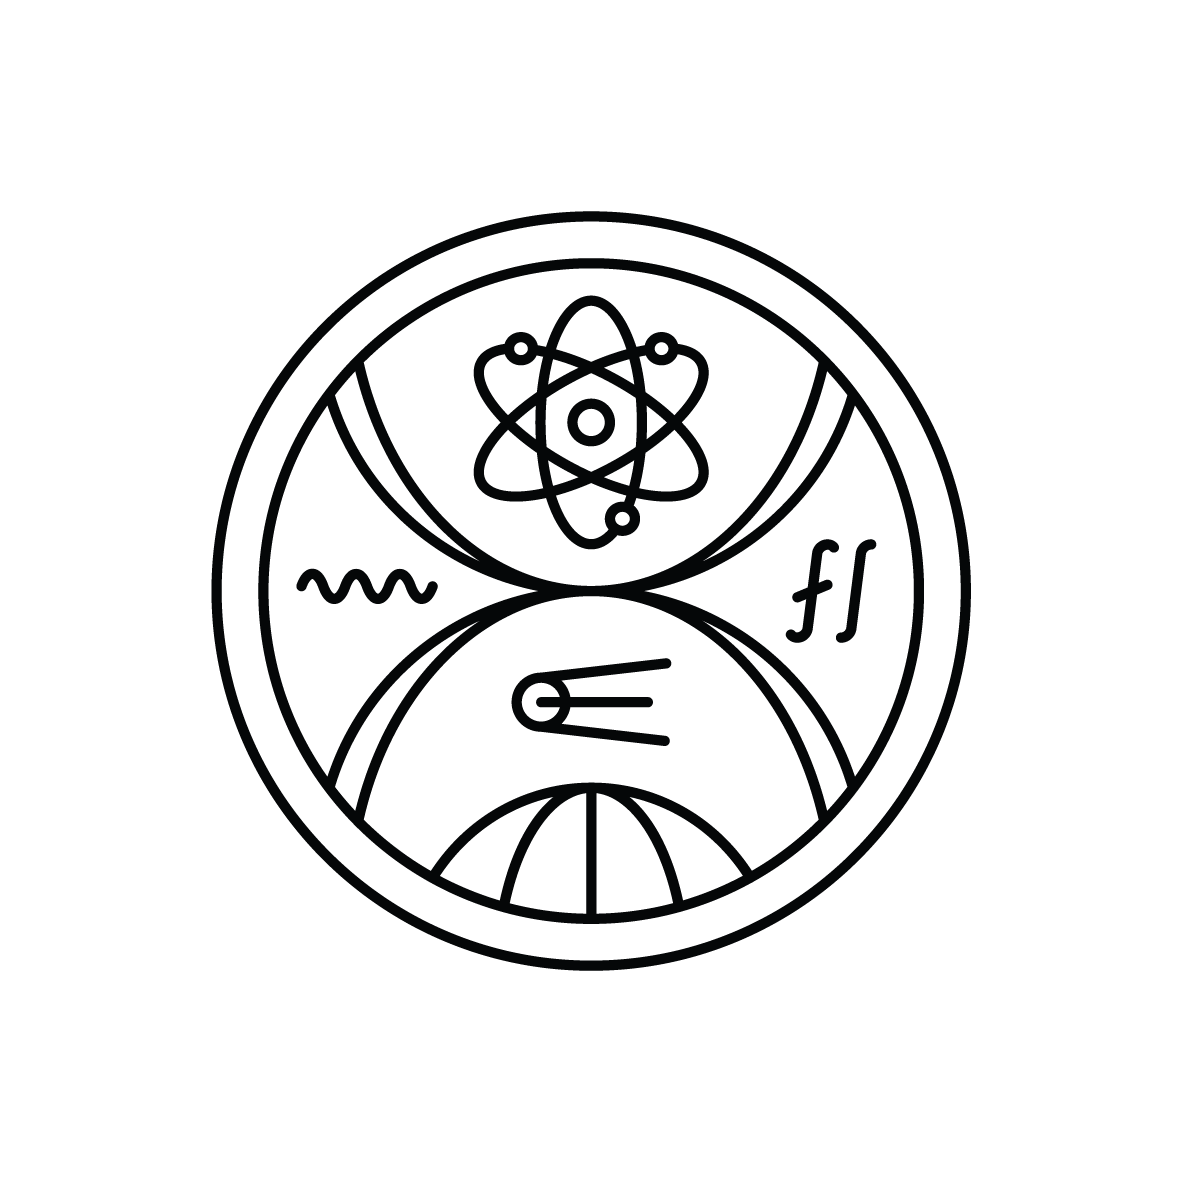
\includegraphics[width=0.4\textwidth]{images/FMFI_logo_BP.png}\label{img:logo}
    \end{center}
\end{figure}
\begin{center}
    \textbf{\MakeUppercase{\Large\mftitle}}\\
    \mfthesistype
\end{center}
\vfill
\mfrok \hfill
\mfauthor
%\eject 
\cleardoublepage
% --- koniec obalky ----



% -------------------
% --- Titulný list
% -------------------
\thispagestyle{empty}
\noindent
\begin{minipage}{\textwidth}
    \begin{center}
        \textbf{\mfuniversity \\
            \mffaculty}
    \end{center}
\end{minipage}

\vfill
\begin{figure}[!hbt]
    \begin{center}
        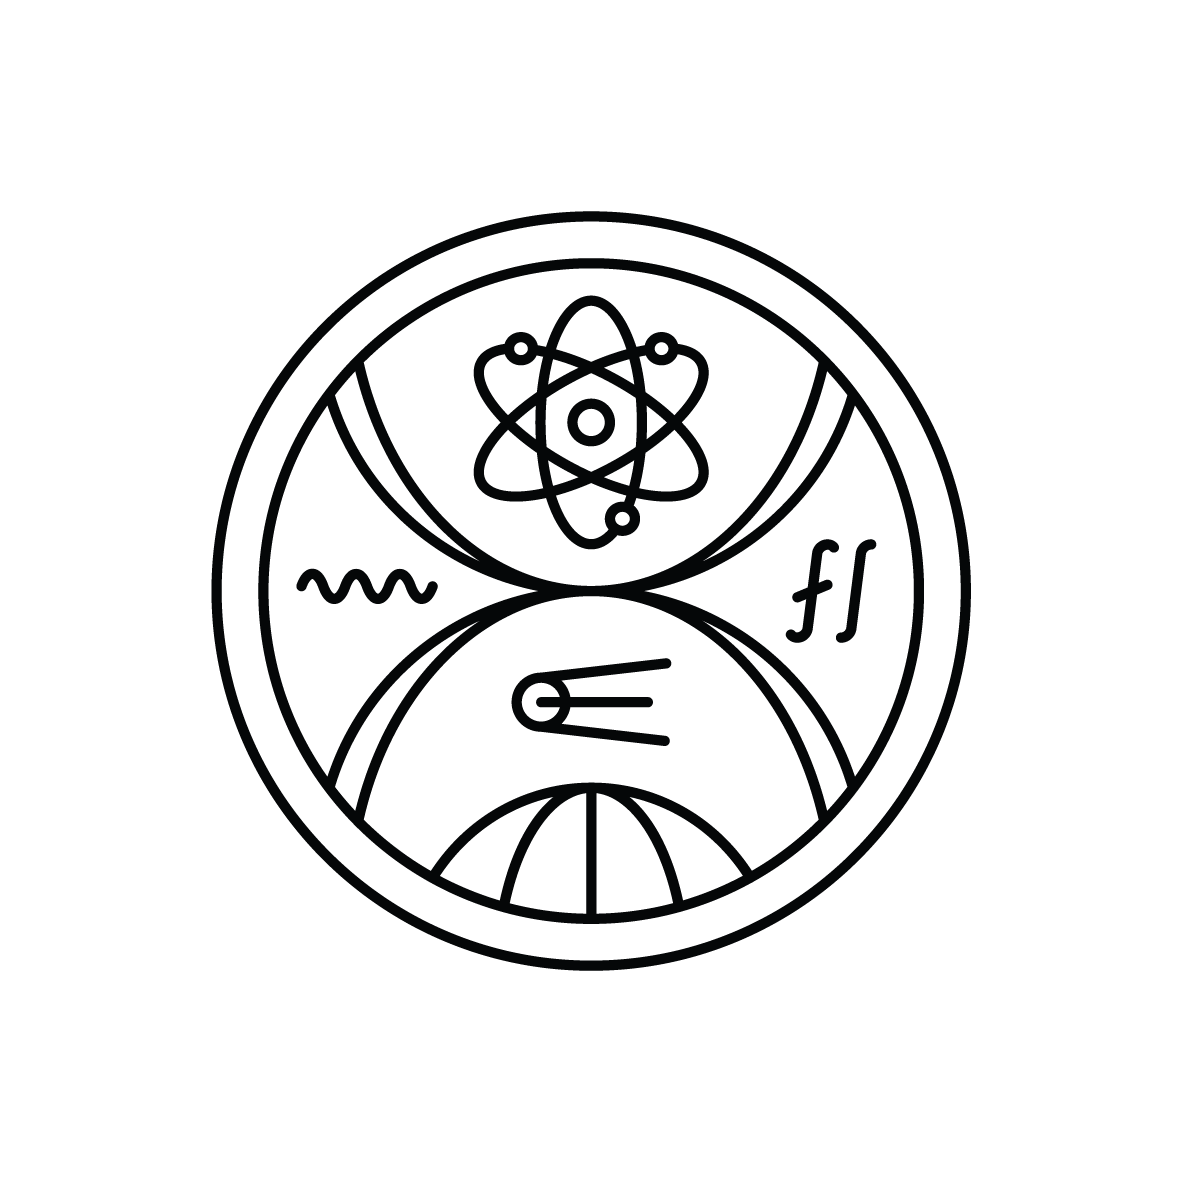
\includegraphics[width=0.4\textwidth]{images/FMFI_logo_BP.png}\label{img:logo_dark}
    \end{center}
\end{figure}

\begin{center}
    \textbf{\MakeUppercase{\Large\mftitle}}\\
    \mfthesistype
\end{center}
\vfill


\begin{tabular}{l l}
    Študijný program:    & \program      \\
    Študijný odbor:      & \mfodbor      \\
    Školiace pracovisko: & \mfpracovisko \\
    Školiteľ:            & \mfskolitel   \\
\end{tabular}

\vfill
\noindent
\mfplacedate \hfill
\mfauthor
%\eject 
\cleardoublepage
% --- Koniec titulnej strany



% -------------------
% --- Zadanie z AIS
% -------------------
% v tlačenej verzii s podpismi zainteresovaných osôb.
% v elektronickej verzii sa zverejňuje zadanie bez podpisov
% v pracach v naglictine anglicke aj slovenske zadanie

\newpage
\thispagestyle{empty}
%\hspace{-2cm}\includegraphics[page=1,width=1.1\textwidth]{zadaniePrace.PDF}

\newpage
\thispagestyle{empty}
%\hspace{-2cm}\includegraphics[page=2,width=1.1\textwidth]{zadaniePrace.PDF}

% --- Koniec zadania


% -------------------
% --- Prehlásenie
% -------------------

{~}\vspace{12cm}

\noindent
\begin{minipage}{0.25\textwidth}~\end{minipage}
\thispagestyle{empty}
\begin{minipage}{0.75\textwidth}
    Čestne prehlasujem, že túto diplomovú prácu som
vypracoval samostatne len s použitím uvedenej literatúry
a za pomoci konzultácií u môjho školiteľa.
\end{minipage}
\vfill
~\hfill {\hbox to 6cm{\dotfill}} \\
\mfplacedate \hfill \mfauthor
\vfill\eject \cleardoublepage
% --- koniec prehlasenia




% -------------------
% --- Poďakovanie
% -------------------
\newpage
\thispagestyle{empty}
\chapter*{Poďakovanie}\label{chap:thank_you}


\vfill\eject
% --- koniec podakovania


% -------------------
% --- Abstrakty
% -------------------
\newpage
\thispagestyle{empty}
\chapter*{Abstrakt}\label{chap:abstract_sk}
Rytmické počítačové hry predstavujú jedinečný žáner, kde hráči interagujú s hrou prostredníctvom preddefinovaných akcií synchronizovaných s hudobným sprievodom. Tieto akcie sú špecifikované v chart súboroch, ktoré sú obvykle vytvárané manuálnym úsilím skúsených umelcov známych ako chart artists. Táto práca sa zaoberá automatizáciou tohto procesu s cieľom demokratizovať tvorbu chartov a umožniť širšej verejnosti prispievať k tvorbe obsahu pre tieto hry.V rámci prehľadu tejto oblasti analyzujeme štruktúry chart súborov v populárnych rytmických hrách a preskúmame existujúce nástroje a literatúru súvisiacu s ich tvorbou. Na základe tejto analýzy navrhujeme a implementujeme algoritmus na automatizované vytváranie grafov, čím skracujeme proces tvorby a otvárame dvere pre nových tvorcov.Experimentálna časť práce sa zameriava na porovnanie kvality automaticky vytvorených chartov so chartami vytvorenými ľudskými umelcami. Na tento účel používame hodnotenia dobrovoľných hráčov, ktorí budú poskytovať spätnú väzbu na základe svojich herných skúseností. Týmto spôsobom hodnotíme efektivitu a presnosť nášho algoritmu voči manuálnej tvorbe.Výsledky tejto práce môžu prispieť k vývoju nových nástrojov na tvorbu obsahu pre rytmické hry a otvárať diskusiu o možnostiach automatizácie v tvorbe herného obsahu v iných žánroch.

\paragraph*{Kľúčové slová:}


\newpage
\thispagestyle{empty}
\chapter*{Abstract}\label{chap:abstract_en}
Rhythmic computer games rely on players executing predefined actions synchronized with accompanying music. These actions are specified in chart files, typically created manually by skilled artists known as chart artists. This work addresses the automation of this process to democratize chart creation and enable a broader community to contribute content to these games. Within the overview of this field, we analyze the structures of chart files in popular rhythmic games and explore existing tools and literature related to their creation. Based on this analysis, we propose and implement an algorithm for automated chart generation, streamlining the creation process and opening the door for new creators. The experimental part of the work focuses on comparing the quality of automatically generated charts with those created by human artists. For this purpose, we utilize evaluations from voluntary players who provide feedback based on their gaming experiences. This approach assesses the effectiveness and accuracy of our algorithm compared to manual creation. The results of this work can contribute to the development of new tools for content creation in rhythmic games and initiate discussions on the possibilities of automation in content creation across different gaming genres.

\paragraph*{Keywords:}


% --- koniec abstraktov


% -------------------
% --- Obsah
% -------------------
\newpage
\tableofcontents

% ---  Koniec Obsahu


% -------------------
% --- Zoznamy tabuliek, obrázkov - nepovinne
% -------------------
\newpage
\listoffigures
\listoftables
% ---  Koniec Zoznamov


\mainmatter

\thispagestyle{empty}
\chapter*{Úvod}\label{chap:uvod}
\chapter{Všeobecný prehľad a teória}\label{chap:teoria}

Umelá inteligencia (UI) zaznamenala za posledných niekoľko desaťročí obrovský rast a vývoj, ktorý posunul hranice možností počítačov. Na čele UI je oblasť počítačového videnia využívajúca konvolučné neurónové siete, ktoré dosahujú prelomové výsledky v úlohách rozpoznávania obrazov a objektov.

V tejto kapitole sa budeme venovať Rytmickym počítačovim hram a teóriám umelej inteligencie a CNN, preskúmame prelomové architektúry VGG [42] a ResNet. Začneme s Rytmickymi počítačovimi hrami s ich strukturou. Potom položením základov neurónovej siete. A na koniec trénovaním neurónovej siete, Forward pass, aktivačnými funkciami a známym algoritmom Backpropagation na prispôsobenie váh, aby sa neurónová sieť mohla učiť.

\section{Rytmické Počítačové Hry a Ich Štruktúra}\label{sec:rytmicke_hry}


Rytmické počítačové hry predstavujú špecifický žáner videohier, kde je kľúčovým aspektom hrateľnosti hudba a rytmus. Hráči v týchto hrách nie sú len pasívnymi pozorovateľmi, ale aktívne interagujú s herným prostredím, pričom ich akcie sú synchronizované s hudobnými prvkami. V týchto hrách hráči často vykonávajú preddefinované akcie, ako sú stlačenia kláves alebo tlačidiel v rytmickom poradí, v súlade s hudbou a vizuálnymi indikáciami na obrazovke.

Kľúčové charakteristiky rytmických počítačových hier zahŕňajú:

\begin{itemize}
\item \textbf{Hudobný Prvok} - Hudba nie je len pozadím, ale aktívne ovplyvňuje hrateľnosť a vizuálny dizajn hry. Hráči reagujú na hudobné prvky, ako sú rytmus a melódia.
\item \textbf{Vizuálne Indikácie} - Na obrazovke sa zobrazujú grafické indikácie alebo symboly, ktoré signalizujú hráčovi, kedy a aké akcie je potrebné vykonať. Vizuálne prvky sú synchronizované s hudobným pozadím.
\item \textbf{Preddefinované Akcie} - Hráči vykonávajú preddefinované akcie, ako sú stlačenia kláves alebo tlačidiel, v súlade s hudbou a vizuálnymi indikáciami na obrazovke.
\item \textbf{Úrovne alebo Levely} - Hry často obsahujú štruktúrované úrovne alebo levely, kde sa obtiažnosť postupne zvyšuje. Hráči dosahujú úspech tým, že dokončujú úrovne s vysokou presnosťou a bodovým skóre.
\end{itemize}

Tieto hry nie len poskytujú zábavu, ale tiež stimulujú hráčové vnímanie hudby a rytmu, vytvárajúc jedinečný zážitok spojením digitálnej zábavy s hudobným umením.

\section{Rôzne typy rytmických počítačových hier}\label{sec:typy}


Rozlíšenie medzi rôznymi typmi rytmických hier môže byť užitočné na porozumenie rôznych prístupov k tomuto žánru. Tu sú niektoré základné typy rytmických hier a ich charakteristiky:

\begin{itemize}

\item \textbf{Tanečné hry} - Hráči tancujú na hudbu a snažia sa napodobniť tanečné kroky, ktoré sú zobrazené na obrazovke, poprípade majú tanečnú podložku, na ktorej sa nachádzajú tlačidlá, na ktoré je potrebné stúpiť keď sa na obrazovke. Príkladom tanečných hier sú \textit{Just Dance} alebo \textit{Dance Dance Revolution}.
\item \textbf{Hry s Nástrojmi} - Hráči hrajú na reálne hudobné nástroje, ako sú gitara alebo klávesy. Hráči musia zahrať správne tóny v správnom čase. Príkladom hier s nástrojmi sú \textit{Guitar Hero} alebo \textit{Rock Band}.
\item \textbf{Hry s Dotykovým Displejom} - Hráči stláčajú tlačidlá alebo podobné objekty na dotykovom displeji. Príkladom hier s dotykovým displejom sú \textit{Beatstar} alebo \textit{osu!}.
\item \textbf{Hry vo Virtuálnej Realite} - Hráči interagujú s roznými objektami v hernom prostredí vo virtuálnej realite. Príkladom hry vo virtuálnej realite je \textit{Beat Saber}.
\end{itemize}

Poslednemu zmieňovanemu typu a hre \textit{Beat Saber} sa budeme venovať v tejto práci. 

\section{Hra Beat Saber}\label{sec:beat_saber}

Beat Saber je hra pre virtuálnu realitu, ktorá bola vyvinutá a vydaná českym herným štúdiom Beat Games. Hra bola v predbežnom prístupe vydaná v máji 2018 a neskôr v máji 2019 bola vydaná ako plná verzia. Hra je dostupná pre platformy PlayStation 4, Windows, Meta Quest a ďalšie. Hráč používa ovládače pre virtuálnu realitu na ovládanie dvoch svetelných mečov, ktoré sú prednastavené na červenú a modrú farbu pre ľavú a pravú ruku. \cite{sutrich2020beatsaber}

V každej pesničke hra hráčovi predkladá postupnosť približujúcich sa blokov súčasne s rytmom hudby, umiestnených v jednej z 12 možných pozícií na mriežke 4x3. Každý blok môže byť označený šípkou, ktorá naznačuje jednu z ôsmich možných smerov, ktorým musí byť blok správne pretnutý. Existujú aj bloky s bodkami namiesto šípiek, ktoré hráči môžu zasiahnuť z akéhokoľvek smeru. Okrem toho sa objavujú aj bomby, ktoré hráč nesmie zasiahnuť, a prekážky v podobe približujúcich sa stien, ktorým sa je potrebné vyhnúť hlavou.

Beat Saber bol dodaný s desiatimi piesňami, ale bol rozšírený niekoľkými balíkmi s obsahom na stiahnutie a aktualizáciami, ktoré zahŕňajú nové piesne. Niekoľko z nich obsahuje originálne skladby, ale niekoľko balíkov obsahuje licencované piesne s hudbou a špeciálnymi úrovňami od rôznych umelcov. Okrem toho komunita vytvorila modifikácie pre Beat Saber, ktoré umožňujú vlastné piesne a mapy.

Počas hry sa objavujú bloky, ktoré majú rôzne špeciálne efekty, ako napríklad blok s vedenou čiarou alebo blok pozostávajúci z viacerých menších blokov. Zároveň má hra veľmi bohato editovateľné vizuálne efekty, ako napríklad laserové show a podobne. V aktuálnej verzii hry sú k dispozícii 5 rôznych herných režimov: Standard, No Arrows (bloky je možné pretnúť v akomkoľvek smere), One Saber (používa sa len jeden meč), 90 Degrees a 360 Degrees (bloky sa približujú v rôznych smeroch).

Hra má tiež niekoľko úrovní obtiažnosti, ktoré sú Easy, Normal, Hard, Expert a Expert+. Tieto úrovne obtiažnosti sa líšia počtom blokov, rýchlosťou približovania sa blokov, počtom prekážok a podobne.

V našej práci sa budeme venovať režimu Standard, ktorý je najpoužívanejší a najviac rozšírený. A zároveň sa budeme venovať trom základným objektom v hre, ktorými sú bloky, prekážky a bomby. Zameriame sa aj na všetky úrovne obtiažnosti, ktoré sú dostupné v hre.

\section{Umelá neurónová sieť}\label{sec:neuronove_siete}

Koncept umelej neurónovej siete (ANN) je voľne inšpirovaný fungovaním ľudského mozgu. Neuróny v ANN sú podobne prepojené a aktivované ako v ľudskom mozgu. ANN prijíma vstupné údaje a prechádza nimi cez aktivačnú funkciu, v dôsledku čoho sa niektoré neuróny v sieti aktivujú a vytvárajú výstup.

Univerzálna aproximačná veta hovorí, že vždy môžeme nájsť dostatočne veľkú neurónovú sieť so správnou sadou váh, ktorá dokáže správne predpovedať akýkoľvek výstup pri akomkoľvek vstupe.

Neurónová sieť sa skladá zo vstupnej, skrytej a výstupnej vrstvy. Ak sú neuróny v každej vrstve prepojené s neurónmi v inej vrstve, potom je neurónová sieť plne prepojená neurónová sieť.  Hodnoty neurónov v sieti závisia od vstupných údajov a pridanej nelinearity. Spojenia medzi neurónmi sú takzvané váhy.

\begin{figure}[H]
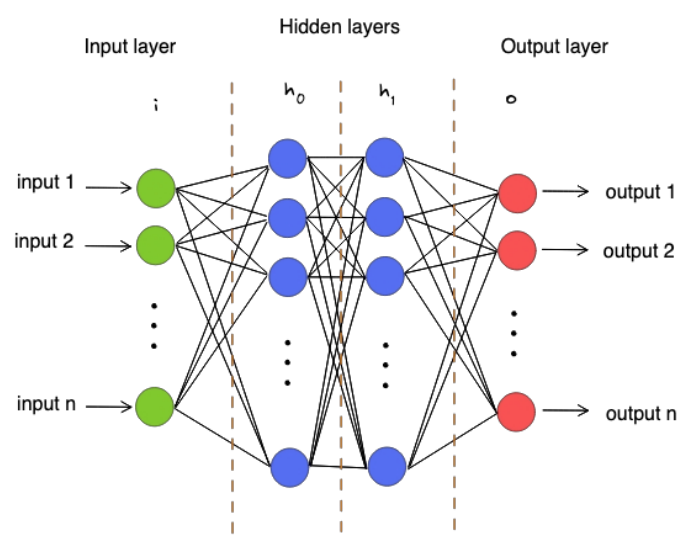
\includegraphics{images/neuronova_siet.png}\label{img:neuronova_siet}
\caption{Ukážka neurónovej siete}
\end{figure}
\subsection{Trénovanie neurónovej siete}\label{subsec:trening}

\subsubsection{Forward pass}\label{subsubsec:forward_pass}

Forward pass je jednou z rozhodujúcich zložiek procesu trénovania neurónových sietí.
Dopredu sa šíriacim spôsobom neurónová sieť vypočítava výstupné predpovede na
základe vstupných údajov. Začína sa na vstupnej vrstve, kde sa prijímajú údaje, a
pokračuje cez každú ďalšiu vrstvu v sieti. Počas tohto prechodu sa vstupné údaje
transformujú prostredníctvom série lineárnych a nelineárnych operácií, ako sú
násobenie matíc a aktivačné funkcie. Tieto transformácie prebiehajú v každej vrstve a
výstup z jednej vrstvy slúži ako vstup pre ďalšiu vrstvu. Posledná výstupná vrstva
generuje predpovede siete. 

Pred začatím trénovania siete sa náhodne vygenerujú hodnoty váh. Pre lepšiu
konvergenciu váh sa odporúča vzorkovať ich z Heovho rozdelenia.

\subsubsection{Stratová funkcia}\label{subsubsec:stratova_funkcia}

Stratová alebo chybová funkcia udáva, ako model funguje. V procese trénovania
neurónových sietí chceme minimalizovať stratovú funkciu úpravou váh siete. Na
výpočet stratovej funkcie zvyčajne potrebujeme anotované hodnoty základných
pravdivých hodnôt. Pre stratovú funkciu môžeme zvoliť jednoduchú strednú
kvadratickú chybu.

Ďalším príkladom stratovej funkcie pre problémy binárnej klasifikácie je binárna
krížová entropia

Pri binárnej klasifikácii sú predpovedané kategórie práve 0 a 1. 

\subsubsection{Backpropagation}\label{subsubsec:backpropagation}

Cieľom algoritmu spätného šírenia je vypočítať deriváciu stratovej funkcie vzhľadom
na každú váhu v sieti. To sa môže použiť v spojení s optimalizačným algoritmom
založeným na gradiente na minimalizáciu stratovej funkcie. Algoritmus začína
od výstupnej vrstvy a prechádza do vstupnej vrstvy. Aby sme vypočítali, ako veľmi prispieva každá váha siete k celkovej chybe, musíme vypočítať gradienty pomocou reťazového pravidla.

\begin{figure}[H]
  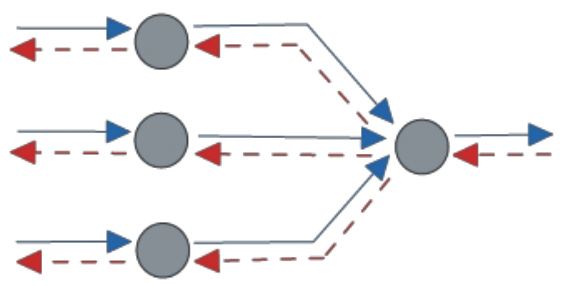
\includegraphics{images/forward_back.png}\label{img:forward_back}
  \caption{Ukážka Forward pass (Modre sipky) a Backpropagation (Cervene sipky)}
\end{figure}

\subsection{Aktivačné funkcie}\label{subsec:aktivacne_funkcie}

Aktivačná funkcia je funkcia, ktorá sa aplikuje na výstup každého neurónu v sieti.
Aktivačná funkcia pridáva do modelu nelinearitu, takže sieť môže aproximovať
takmer akúkoľvek funkciu. Ak sa aktivačná funkcia do siete nezapracuje, model bude
môcť vykonávať len lineárnu klasifikáciu

\subsubsection{Sigmoid}\label{subsubsec:sigmoid}

Sigmoid je aktivačná funkcia, ktorá je definovaná ako $\sigma(x) = \frac{1}{1 + e^{-x}}$. Táto funkcia je spojitá a diferencovateľná, čo je dôležité pre algoritmus. Táto aktivačná funkcia sa používala v začiatkoch. Aktivačná funkcia však stláča
výstup na rozsah medzi [0, 1]. Výsledkom je sigmoida
výstup funkcie sa nasýti pri vysokých a nízkych vstupných hodnotách, čo má za
následok problém miznúceho gradientu. Problém miznúceho gradientu sa vzťahuje na situáciu,
keď sa gradient účelovej funkcie týkajúci sa parametra blíži k nule, čo spôsobuje malé
aktualizácie parametrov počas trénovania siete pomocou metódy stochastického
zostupu po gradiente. To má za následok nedostatočné zmeny parametrov siete, a sieť
sa tak nedokáže správne učiť. Okrem toho neprítomnosť nulového výstupu prispieva k
suboptimálnej konvergencii.

\subsubsection{ReLU}\label{subsubsec:relu}

ReLU je aktivačná funkcia, ktorá je definovaná ako $f(x) = max(0, x)$. Táto funkcia je spojitá, ale nie je diferencovateľná v bode x = 0. Táto funkcia je v súčasnosti najpoužívanejšia aktivačná funkcia. ReLU je jednoduchá na výpočet a má výhodu, že sa nenasýti pri vysokých vstupných hodnotách. ReLU však môže mať problém s mŕtvymi neurónmi. Mŕtvy neurón je neurón, ktorý má všetky váhy nastavené na záporné hodnoty. V tomto prípade sa výstup neurónu vždy rovná 0 a gradient je vždy 0. To znamená, že neurón sa už nikdy nebude učiť, pretože sa nikdy neaktualizujú jeho váhy. Tento problém sa dá vyriešiť použitím variantu ReLU, ktorý sa nazýva Leaky ReLU. Leaky ReLU je definovaná ako $f(x) = max(0.01x, x)$.

\subsubsection{Softmax}\label{subsubsec:softmax}

Softmax je aktivačná funkcia, ktorá je definovaná ako $\sigma(x)_i = \frac{e^{x_i}}{\sum_{j=1}^{K} e^{x_j}}$. Táto funkcia je spojitá a diferencovateľná. Táto funkcia sa používa na klasifikáciu viacerých tried. Výstup tejto funkcie je vždy v rozsahu [0, 1] a súčet výstupov je vždy 1. Táto funkcia sa používa na klasifikáciu viacerých tried. Výstup tejto funkcie je vždy v rozsahu [0, 1] a súčet výstupov je vždy 1. Táto funkcia sa používa na klasifikáciu viacerých tried. Výstup tejto funkcie je vždy v rozsahu [0, 1] a súčet výstupov je vždy 1.

\section{Optimalizačné algoritmy}\label{sec:optimalizacne_algoritmy}

Optimalizačné algoritmy sa používajú na minimalizáciu stratovej funkcie. V tejto
sekcii sa budeme venovať niektorým základným optimalizačným algoritmom.

\subsection{Stochastický zostup po gradiente}\label{subsec:stochastic_gradient_descent}

Stochastický zostup po gradiente (SGD) je najzákladnejší optimalizačný algoritmus.
SGD je iteratívny algoritmus, ktorý sa používa na minimalizáciu stratovej funkcie.
Algoritmus začína náhodným výberom počiatočných váh. Potom sa vypočíta gradient
stratovej funkcie vzhľadom na každú váhu v sieti. Váhy sa aktualizujú v smere
gradientu stratovej funkcie. Tento proces sa opakuje, kým sa váhy nemenia alebo
kým sa nedosiahne maximálny počet iterácií.

\subsection{Momentum}\label{subsec:momentum}

Momentum je optimalizačný algoritmus, ktorý sa používa na minimalizáciu stratovej
funkcie. Tento algoritmus je podobný SGD, ale má výhodu, že sa môže vyhnúť lokálnym
minimám. Tento algoritmus používa koncept momentum, ktorý je definovaný ako
exponenciálny pohyblivý priemer gradientov. 

\subsection{Adam}\label{subsec:adam}

Adam je optimalizačný algoritmus, ktorý sa používa na minimalizáciu stratovej
funkcie. Tento algoritmus je kombináciou algoritmov RMSProp a Momentum. Tento
algoritmus používa koncept exponenciálneho pohyblivého priemeru gradientov a
exponenciálneho pohyblivého priemeru druhých momentov gradientov.

\section{Konvolučná neurónová sieť}\label{sec:cnn}

Konvolučná neurónová sieť (CNN) je špeciálna viacvrstvová neurónová sieť pre
priestorové údaje. Tradičná CNN sa skladá z jednej alebo viacerých konvolučných
vrstiev, vrstiev združovania, po ktorých nasleduje jedna alebo viacero plne
prepojených vrstiev a na konci je výstupná vrstva.

\begin{figure}[H]
  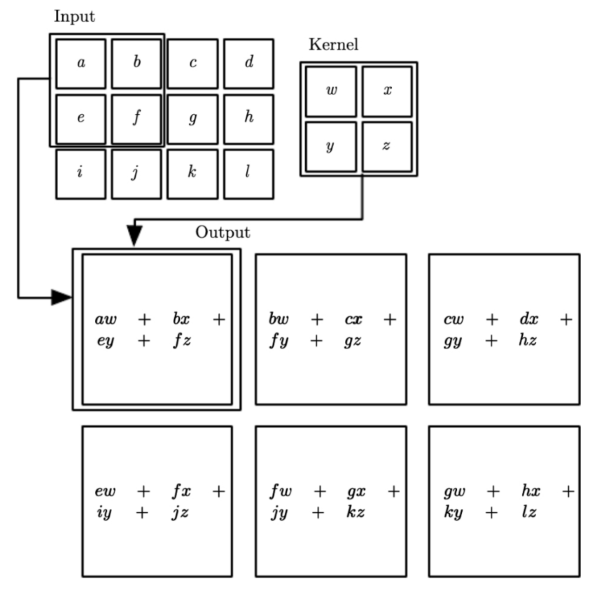
\includegraphics{images/konvolucia.png}\label{img:cnn}
  \caption{Príklad operácie 2D konvolúcie. Štvorce so šípkami znázorňujú, ako
  bol vypočítaný ľavý horný prvok výstupnej matice po aplikácii jadra na príslušnú ľavú
  hornú oblasť vstupnej matice.}
\end{figure}

\subsection{Konvolučná vrstva}\label{subsec:konvolucna_vrstva}

Konvolučná vrstva je základným stavebným kameňom CNN. Pozostáva z
konvolučného jadra (filtrov). Jadro sa konvolúciou spája so vstupnými údajmi, čo
vedie k extrakcii príznakov uložených v mape príznakov. Jadro možno opísať ako
maticu s naučenými hodnotami, ktoré sú známe ako
váha jadra. Príklad 2D jadra na obrázku 1.5. V procese trénovania sa váhy jadra
CNN aktualizujú, čím sa zo vstupu extrahujú ďalšie podstatné vlastnosti.
Na extrakciu príznakov zo vstupného obrazu sa vykonáva operácia konvolúcie.
Operácia sa začína v ľavom hornom rohu vstupnej matice. Jadro je posunuté
horizontálne aj vertikálne. Po každom posune sa vykoná bodový súčin vynásobením a
sčítaním príslušných hodnôt v jadre a vstupnom obraze a vytvorí sa jedna skalárna
hodnota na výstupe mapy príznakov.

Konvolučná vrstva má ďalšie dva parametre. Prvým je krok, ktorý definuje krok
posunu jadra, a druhým je výplň. Vypĺňanie rieši problém rýchlo stráca informácie o prvkoch na okrajoch obrázkov. Padding je pridávanie núl
okolo obrazu, zväčšovanie vstupnej veľkosti a pridávanie ďalších informácií o prvkoch
na hraniciach do výslednej mapy prvkov.

Použitím operácie konvolúcie na vstupné údaje (obrázok, audio) sa zmenia rozmery
vstupných údajov. Táto zmena závisí od veľkosti jadra, kroku a výplne (padding).

\subsection{Pooling vrstva}\label{subsec:pooling_vrstva}

Pooling vrstvy sa bežne vkladajú medzi konvolučné vrstvy. Pooling vrstva
teda sumarizuje prvky v oblasti mapy prvkov vytvorenej predchádzajúcou
konvolúciou vrstvy. Nasledujúce výpočty sa teda vykonávajú na zosumarizovaných
prvkoch namiesto presne umiestnených prvkov vytvorených konvolučnou vrstvou.
Tento proces zabezpečuje väčšiu odolnosť modelu voči zmenám polohy prvku vo
vstupnom obraze. Keďže združovacia vrstva sumarizuje prvky, znižuje priestorové
rozmery.
Existujú tri hlavné operácie poolingu: priemer, maximum a globálne
združovanie. Priemerny pooling berie priemernú hodnotu z pooling filtra.

Max pooling má rovnaký postup, ale berie maximálnu hodnotu.

Globálny priemerny pooling sa používa na redukciu trojrozmerných máp prvkov na jednorozmerné vektory.

\begin{figure}[H]
  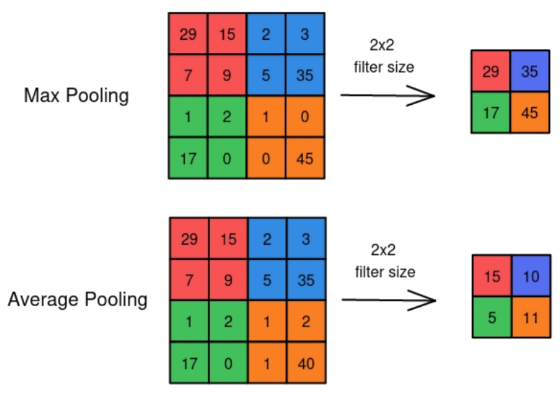
\includegraphics{images/pooling.png}\label{img:max_pooling}
  \caption{Príklad MAX poolingu (hore), príklad priemerného poolingu (dole)}
\end{figure}

\begin{figure}[H]
  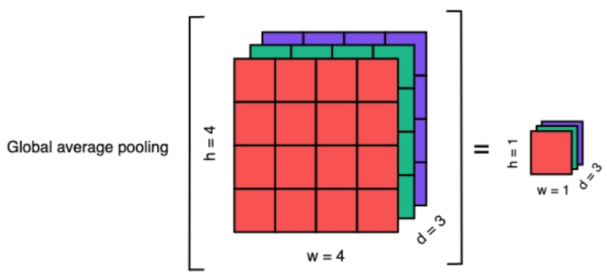
\includegraphics{images/global_pooling.png}\label{img:global_pooling}
  \caption{Príklad globalneho poolingu}
\end{figure}

\subsection{Plne prepojená vrstva}\label{subsec:plne_prepojena_vrstva}

Posledným stupňom konvolučnej neurónovej siete je plne prepojená vrstva. V tejto
vrstve sú neuróny navzájom prepojené. Táto vrstva sa používa napríklad na
klasifikáciu objektov na vstupnom obraze na základe extrahovaných funkcií z
predchádzajúcich vrstiev, v našom prípade konvolučných vrstiev.




\thispagestyle{empty}
\chapter*{Záver}\label{chap:zaver}


%main content 


% -------------------
% --- Bibliografia
% -------------------

\backmatter

\nocite{*}
\bibliographystyle{plain}
\bibliography{references}

%---koniec bibliografie

\end{document}